% !TEX root = ../main.tex
%% ---------------------------------------------------------------------------
% 4.1 Examination for integration consistency
%% ---------------------------------------------------------------------------

\subsection{Examination for integration consistency}\label{sec:consistency}

As stated in Section \ref{sec:error}, the integration consistency of an integration method plays a crucial role in the convergence performance.
Consequently, for subsequent development, we investigate and examine the integration consistency by manufactured problems with polynomial solutions:
\begin{equation}\label{manufactured}
w=\left(\sum_{i=1}^{n_{sd}}x_i+1\right)^{p}
\end{equation}

\begin{figure}[pos=htbp]
\centering
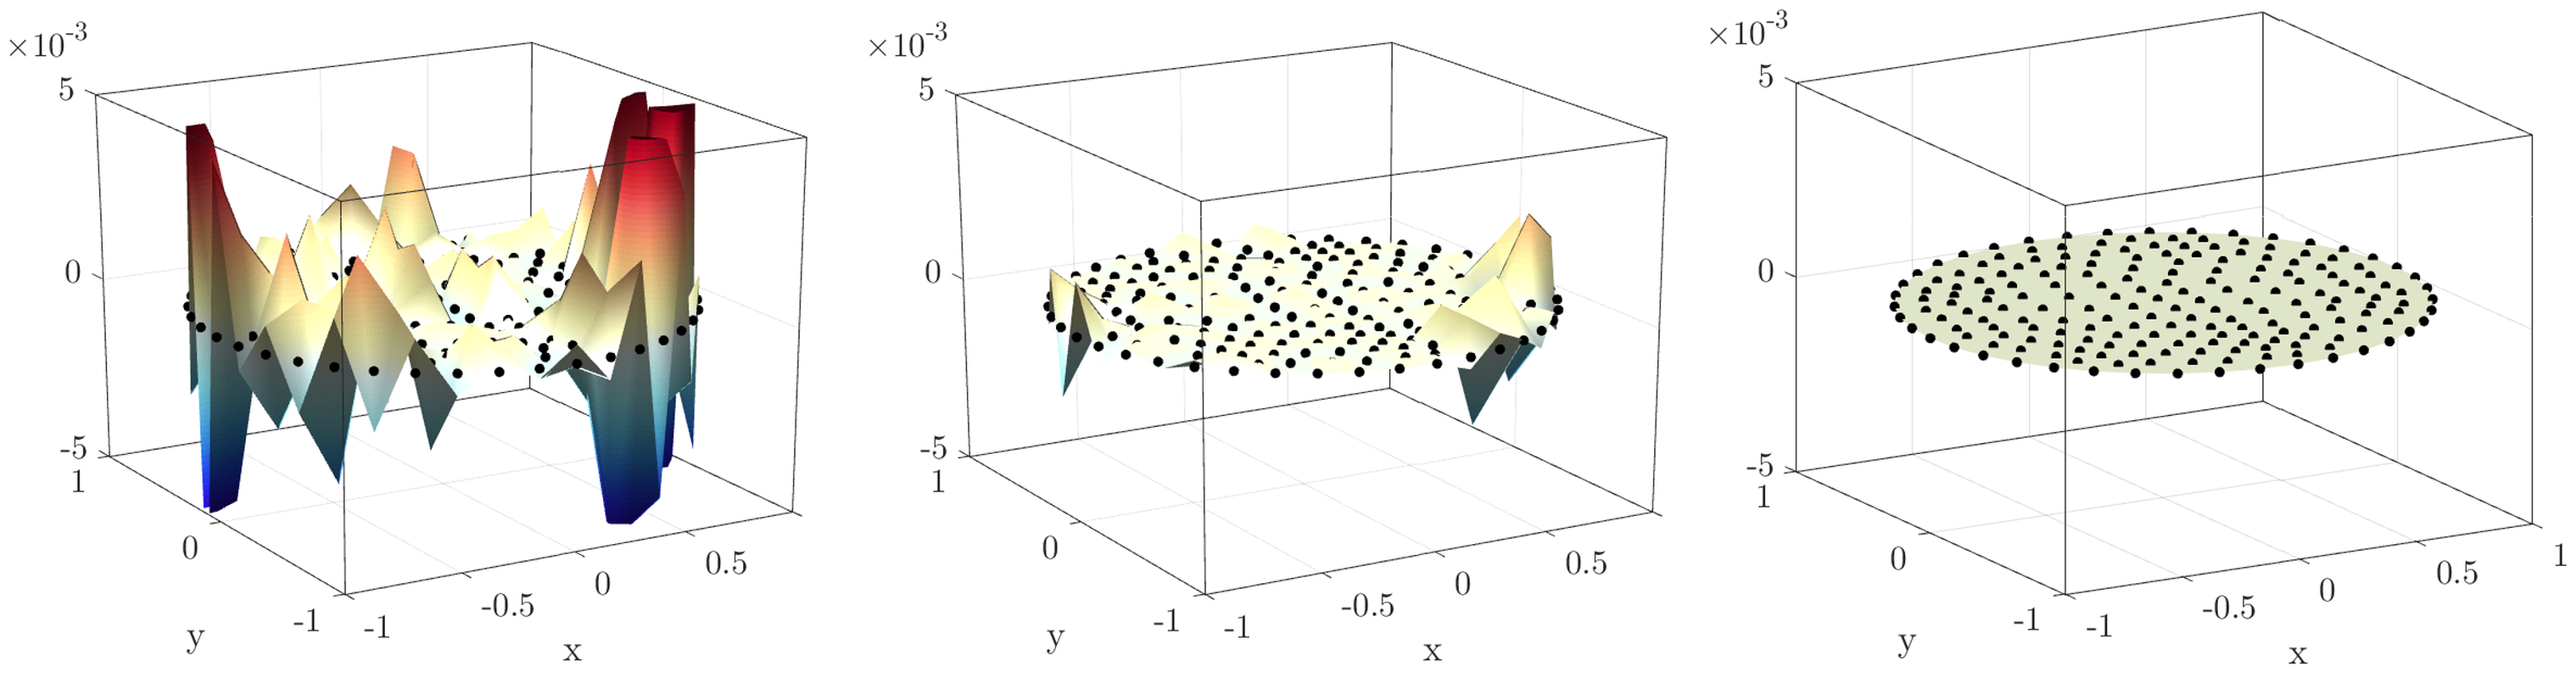
\includegraphics[width=\textwidth]{figs/fig01.png}
\caption{Examination of the 2nd order integration consistency for 2D cubic meshfree formulation.}\label{fig:1}
\end{figure}

\begin{figure}[pos=htbp]
\centering
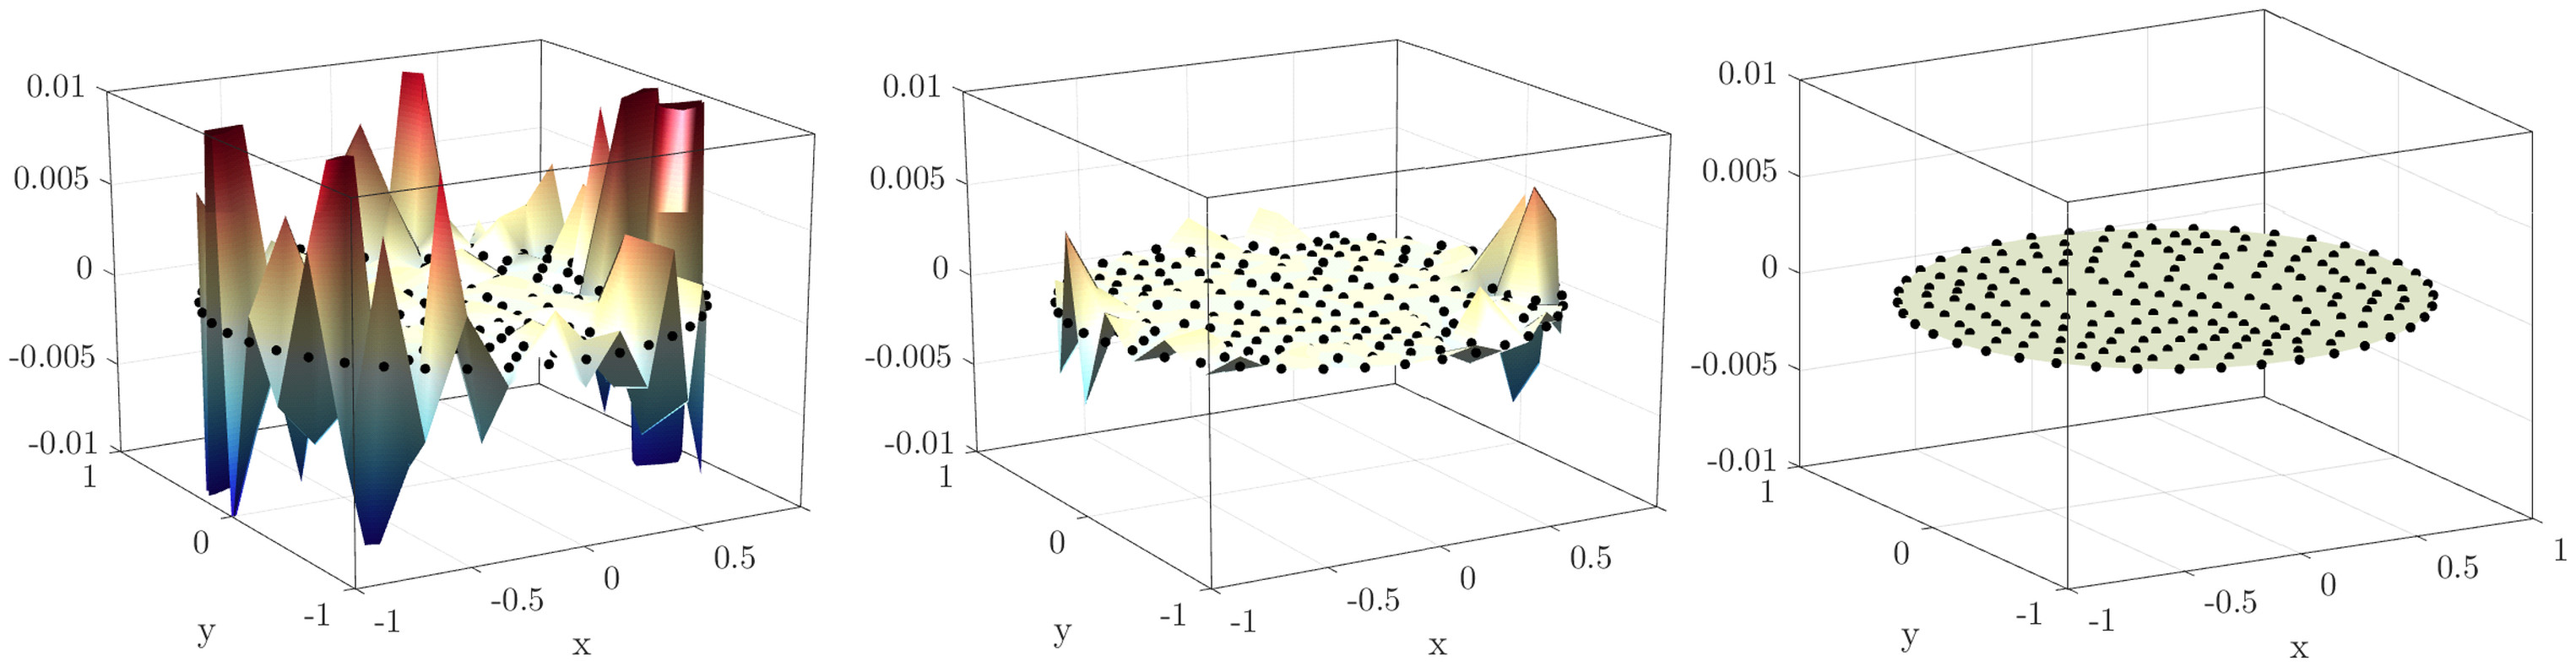
\includegraphics[width=\textwidth]{figs/fig02.png}
\caption{Examination of the 3rd order integration consistency for 2D cubic meshfree formulation.}\label{fig:2}
\end{figure}

\begin{figure}[pos=htbp]
\centering
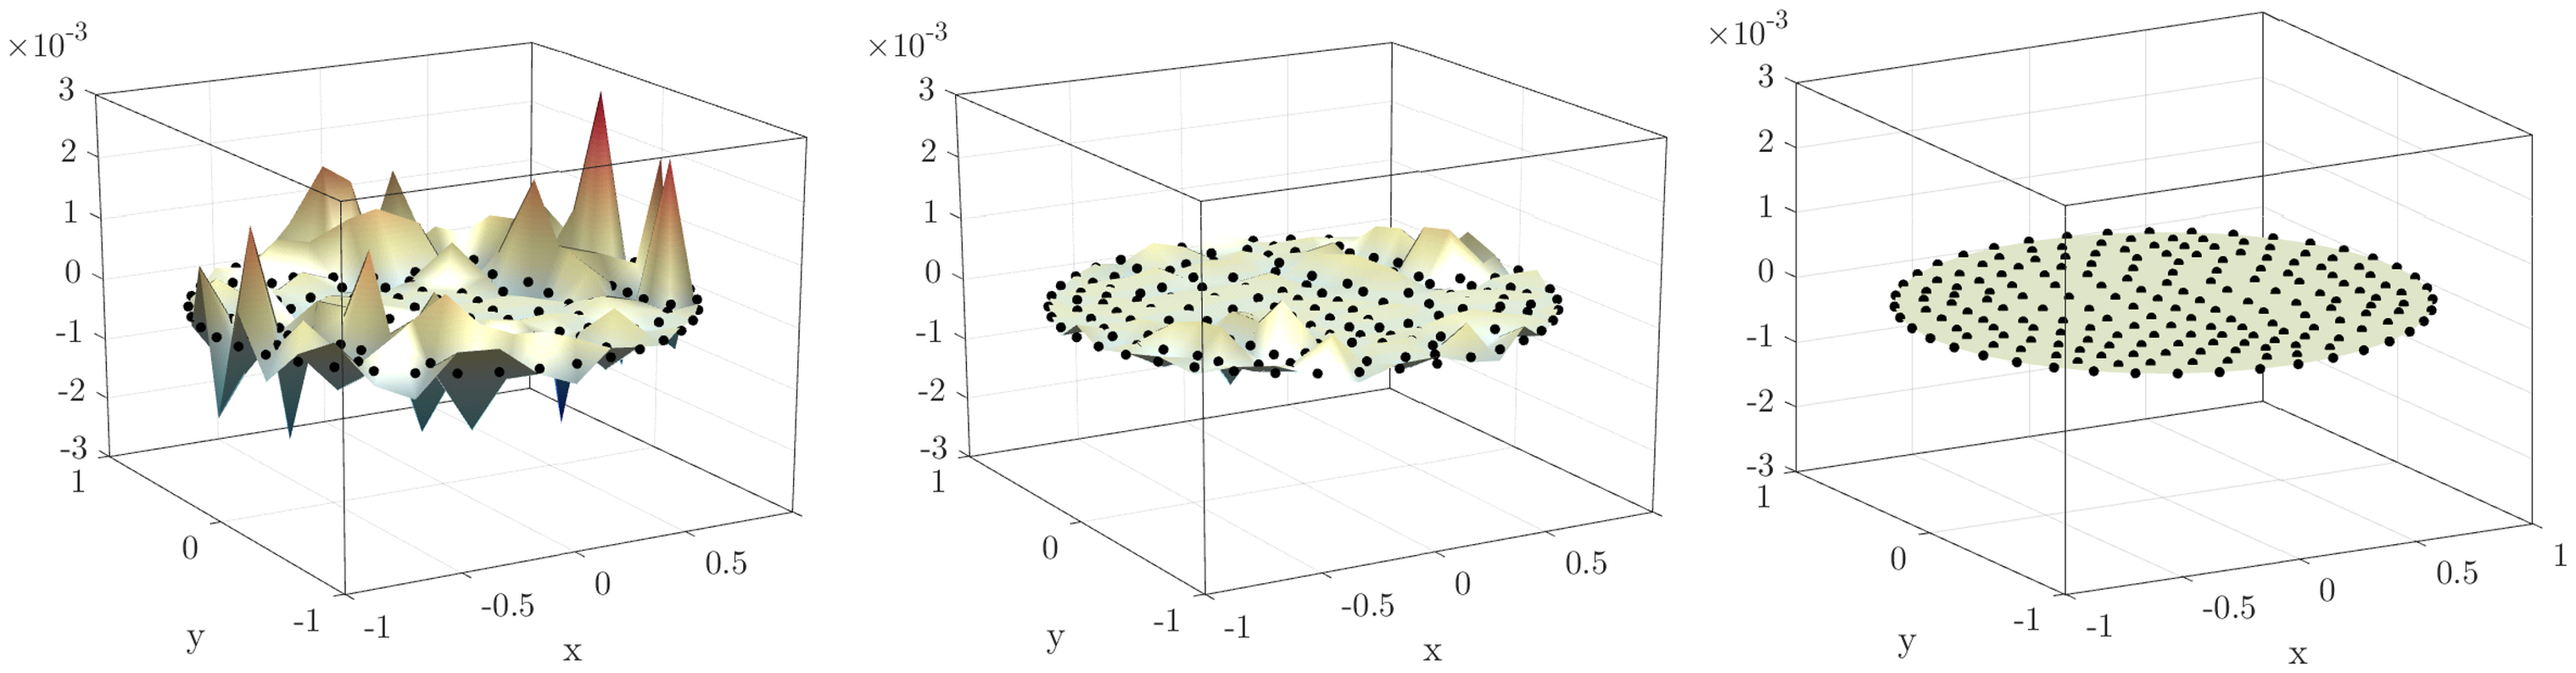
\includegraphics[width=\textwidth]{figs/fig03.png}
\caption{Examination of the 3rd order integration consistency for 2D quartic meshfree formulation.}\label{fig:3}
\end{figure}

\begin{figure}[pos=htbp]
\centering
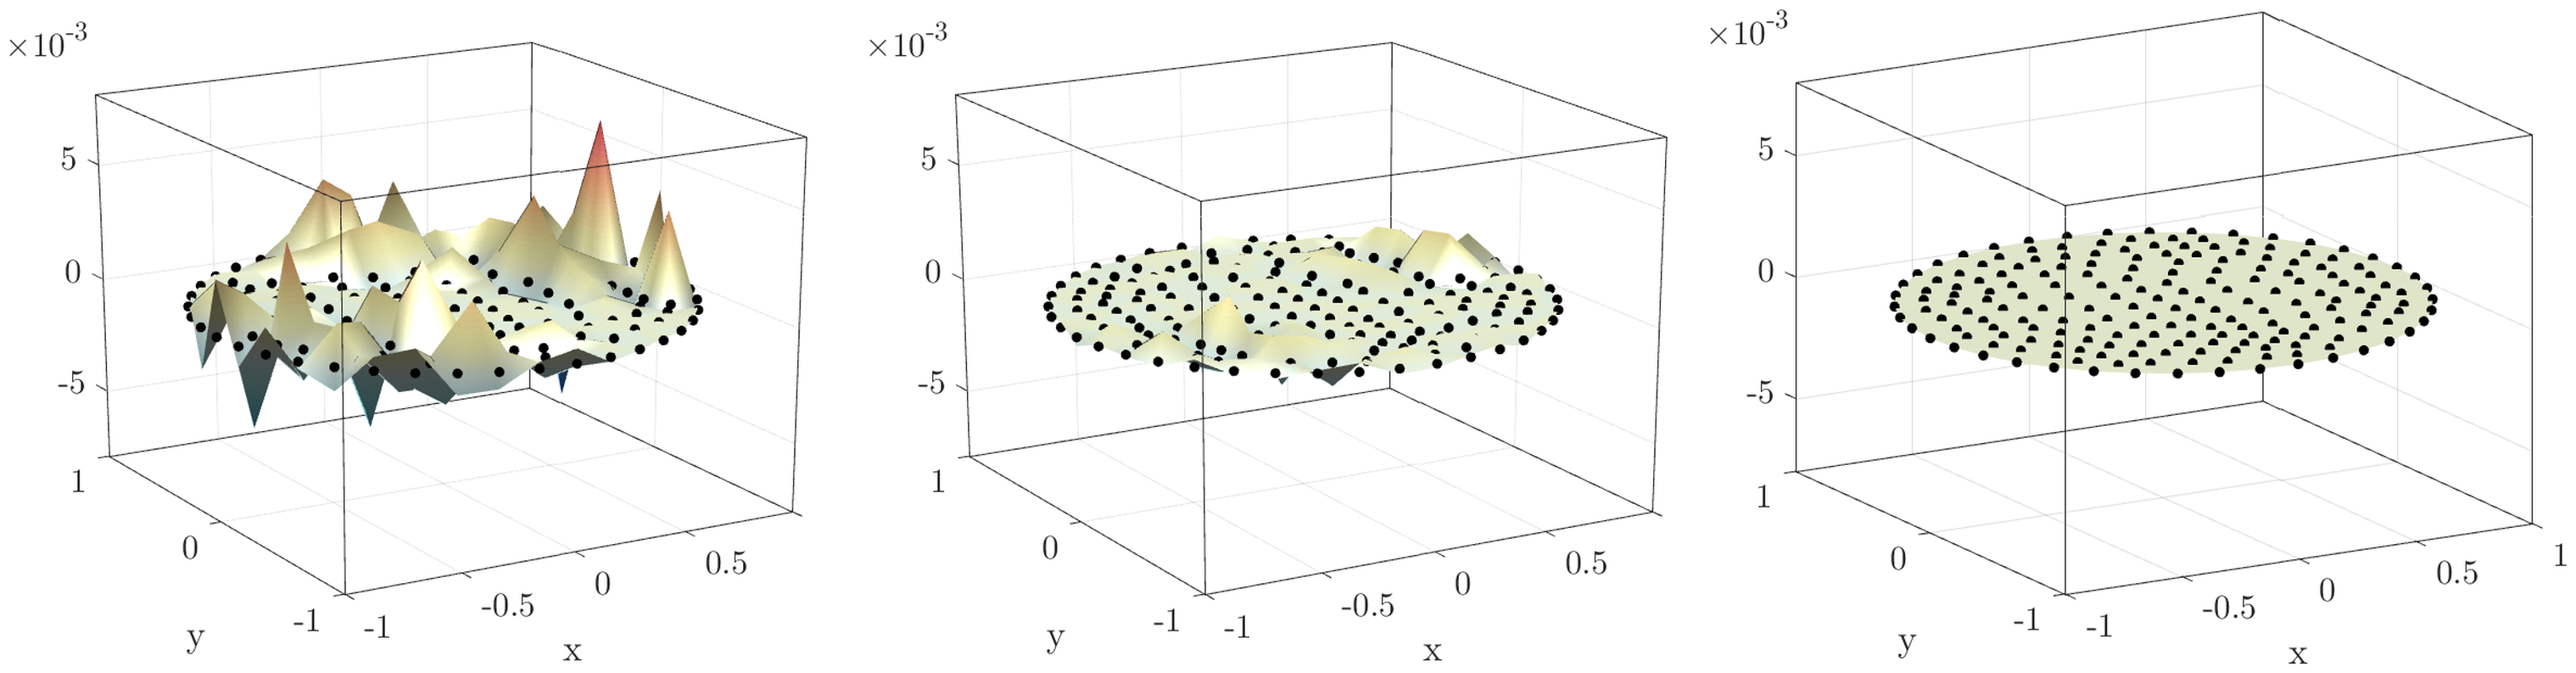
\includegraphics[width=\textwidth]{figs/fig04.png}
\caption{Examination of the 4th order integration consistency for 2D quartic meshfree formulation.}\label{fig:4}
\end{figure}

Figs. \ref{fig:1}--\ref{fig:4} clearly show the various orders of integration consistency of GI and RKGSI for cubic and quartic basis function.
Since RKGSI was generated from integration constraints of weak forms regarding to various orders $q$ of meshfree formulations, it naturally possess the integration consistency the same degree of basis functions.
